\documentclass[aps,prb,twocolumn,superscriptaddress,floatfix,longbibliography]{revtex4-2}

\usepackage{amsmath,amssymb} % math symbols
\usepackage{bm} % bold math font
\usepackage{graphicx} % for figures
\usepackage{comment} % allows block comments
%\usepackage{ulem} % allows strikeout text, e.g. \sout{text}

\usepackage{minted} % allows colored code
\usepackage{textcomp} % This package gives the text quote '

\usepackage{enumitem}
\setlist{noitemsep,leftmargin=*,topsep=0pt,parsep=0pt}

\usepackage{xcolor} % \textcolor{red}{text} will be red for notes
\definecolor{lightgray}{gray}{0.6}
\definecolor{medgray}{gray}{0.4}

\usepackage{hyperref}
\hypersetup{
colorlinks=true,
urlcolor= blue,
citecolor=blue,
linkcolor= blue,
% bookmarks=true,
% bookmarksopen=false,
}

% Code to add paragraph numbers and titles
\newif\ifptitle
\newif\ifpnumber
\newcounter{para}
\newcommand\ptitle[1]{\par\refstepcounter{para}
{\ifpnumber{\noindent\textcolor{lightgray}{\textbf{\thepara}}\indent}\fi}
{\ifptitle{\textbf{[{#1}]}}\fi}}
\ptitletrue  % comment this line to hide paragraph titles
\pnumbertrue  % comment this line to hide paragraph numbers

% minimum font size for figures
\newcommand{\minfont}{6}

% Uncomment this line if you prefer your vectors to appear as bold letters.
% By default they will appear with arrows over them.
% \renewcommand{\vec}[1]{\bm{#1}}

% Allows to rewrite the same title in the supplement
\newcommand{\mytitle}{How 2 Write a Paper and Format it Using \LaTeX}

\begin{document}

\title{\mytitle}

\author{Jennifer E. Hoffman}
\email[]{jhoffman@physics.harvard.edu}
\affiliation{Department of Physics, Harvard University, Cambridge, Massachusetts 02138, USA}
\affiliation{School of Engineering \& Applied Sciences, Harvard University, Cambridge, Massachusetts 02138, USA}

\date{\today}

\begin{abstract}
The goal of this document is to demonstrate how to write a paper. We walk through the process of outlining, writing, formatting in \LaTeX, making figures, referencing, and checking style and content. Source files are available at: \url{http://hoffman.physics.harvard.edu/example-paper/}.
\end{abstract}

\maketitle
\section{\label{sec:Start}Getting Started}

\ptitle{Start writing while you experiment} You should start writing your paper \textit{while} you are working on your experiment. Prof.\ George Whitesides says: ``A paper is not just an archival device for storing a completed research program; it is also a structure for planning your research in progress. If you clearly understand the purpose and form of a paper, it can be immensely useful to you in organizing and conducting your research. A good outline for the paper is also a good plan for the research program. You should write and rewrite these plans/outlines throughout the course of the research. At the beginning, you will have mostly plan; at the end, mostly outline. The continuous effort to understand, analyze, summarize, and reformulate hypotheses on paper will be immensely more efficient for you than a process in which you collect data and start to organize them only when their collection is `complete' .'' Here are some concrete steps to get started.

\begin{enumerate}
\item Read George Whitesides' ``How to Write a Paper'' \cite{WhitesidesAdvMat2004}.

\item Read through \emph{at least} one full paper in your target journal, to get a sense of the content and writing style.

\item To clarify in your own head the purpose of your paper, start by drafting your abstract \cite{NatureAbstract}.

\item Before you tackle the body of the paper, sketch block outlines of the figures. Decide what images and plots you will put in the paper, and how the panels will be arranged. An excellent example of an outline with sketched figures is shown in Ref.\ \cite{GardeziOutline2}, and can be compared to the final published paper in Ref.\ \cite{Gardezi2DMat2020}.

\item Outline at the paragraph level before you write. Look at how many paragraphs there will be in the style of paper you are trying to write. For example, for a standard 4-page scientific letter, aim for 13 paragraphs (generally, you can estimate about 200 words per paragraph). Figure out how to tell your entire story (not numbers, just story!) in 13 stand-alone sentences.

\item Make each of those sentences into the first sentence of a paragraph, and fill into each paragraph only details that are relevant to that first sentence. If you find yourself writing details about the figures, cut and paste them into the captions.

\item If you think of references as you go, you can include the minimal identifying information in parentheses to trigger your memory later, e.g.\ ``(WhitesidesAdvMat)'', so all of the information is compact.

\item Dig into the existing literature to write the intro paragraphs. A thorough literature search may take a full focused week for each intro paragraph. Use an organized, three-pass approach to keep a good balance between depth and breadth of your search \cite{KeshavSIGCOMM2007}.

\item Rewrite your abstract, taking into account what you have learned from the process of writing the paper. As you fine-tune your abstract, refer again to Nature's instructions for writing an abstract \cite{NatureAbstract} and for clear communication more generally \cite{NatNeuro2000}.
\end{enumerate}
\vspace{2mm}

\ptitle{Formatting matters} As you contemplate the paper you have just written, put yourself in the shoes of the reviewers (including your collaborators). You already work many, many hours/week, and you don't really want to spend more time reading this paper. So you're going to be very happy if the figures are pretty, the text flows logically, the references are hyperlinked for easy access, and you can understand the paper quickly. But you're going to be very grumpy if you can't get the main points of the paper from scanning through the figures \& captions. You're going to be even grumpier if you invest time in reading the paper but you still can't get it. Your evaluation of this paper is likely to be swayed by your ease of understanding, regardless of the scientific merits of the work. (See Ref.\ \onlinecite{Kahneman2011} for more information on how formatting, even as simple as font choice, will influence the reader's ``cognitive ease'' and ultimately their judgment of the report.) Down the road, consider a reader who might cite the paper and launch you to fame and glory: the potential citer's decision will be influenced by their ability to easily understand your paper.

\ptitle{Fractal} \textbf{Your paper should be fractal.} Somebody with one minute to look at it should be able to get the main idea just from reading the abstract. Somebody with 5 minutes should be able to look at the figures and get more out of it. Somebody with 10 minutes should be able to get the story from the introduction, first sentence of each paragraph, and conclusion.

\section{\label{sec:LaTeX}\LaTeX}

\ptitle{Intro to \LaTeX} \LaTeX\ is a formatting language that allows professional, publication-quality presentation of scientific text, equations, figures, and hyperlinked references. REVTeX is a specific set of \LaTeX\ macro packages assembled by the American Physical Society (APS) to standardize manuscript formatting for the various Physical Review journals. The APS author website \cite{PhysicalReview} lists acceptable submission formats as: REVTeX \textbf{(preferred)}, \LaTeX, or MSWord. It is sensible to draft your paper in \LaTeX/REVTeX from the beginning. You will need a reference manager, a text editor, and a \LaTeX\ compiler. Typically, you will be working closely with other authors, so you should pick a platform that enables simple sharing and collaborative workflow.

\ptitle{Overleaf} Here we recommend the online \LaTeX\ compiler Overleaf (\url{http://www.overleaf.com/}) for text editing and compiling. Overleaf (formerly known as Share\LaTeX) is an online platform that is great for collaborative writing: it tracks changes and even has a real-time chat function. Note that LyX is a WYSIWYG (what you see is what you get) \LaTeX\ editor that may seem tempting if you initially find tex formatting daunting, but LyX may come back to bite you in the long run, because it hides the guts of the tex code from the user, making it harder to control formatting details.

\begin{raggedright}
\begin{enumerate}
\item Choose \& install a reference management software such as Mendeley:
\url{http://www.mendeley.com/}\\
(See appendix \ref{app:Mendeley} for usage tips.)
\item Make an account on Overleaf:
\url{http://www.overleaf.com/}\\
\item Download the source files for this example paper \cite{HoffmanExample}.
\item Copy the tex and bib files into a new overleaf project, and share with your collaborators.
\end{enumerate}
\end{raggedright}
\vspace{2mm}

\ptitle{Alternatives} Alternatively, you may prefer to run \LaTeX\ directly on your own laptop. In that case, follow the steps below:
\begin{raggedright}
\begin{enumerate}
\item Choose \& install a reference management software:
\begin{itemize}
\item Mendeley: \url{http://www.mendeley.com/}
\item Papers: \url{http://www.papersapp.com/}
\item Endnote: \url{http://www.endnote.com/}
\end{itemize}
\item Download \& install a \LaTeX\ compiler such as MikTex: \\
\url{http://miktex.org/}
\item Download \& install REVTeX 4-2 (see appendix \ref{app:REVTeX}):\\
\url{http://authors.aps.org/revtex4/}
\item Pick an editor such as WinEdt:
\url{http://www.winedt.com/}\\
(You may need to request a university license; may require $\sim 24$ hour turnaround.)
\item Download the source files for this example paper \cite{HoffmanExample}, open the tex and bib files in WinEdt, and get started writing!
\end{enumerate}
\end{raggedright}
\vspace{2mm}

\ptitle{Maintain your outline} It's important not to lose sight of your outline, as you fill in the details of your paper. This \LaTeX\ template file allows you to title each paragraph using the {\tt \textbackslash ptitle\{\}} command. You should keep these titles in place throughout the entire paper-writing process; they will serve as a constant reminder to keep each paragraph focused on a single point. You should be able to skim through these bold paragraph titles, without reading any of the intervening sentences, and still understand the basic logical flow of the paper. At the final step before submission, comment out the line {\tt \textbackslash ptitletrue} in the header, to hide the paragraph titles. But do not delete the paragraph titles, because they will remain useful to you in the inevitable paper revision process down the road!

\section{\label{sec:Formatting}Formatting}

\ptitle{Formatting checklist} Whether you are using a compiler on your computer or online, please use the latest version of REVTeX, and check your formatting carefully.
\begin{itemize}[label=$\Box$]
\item Check math \& symbolic formatting, as in Table \ref{tab:mathformat}.
\begin{table}[h!]
  \begin{center}
    \caption{Formatting mathematical symbols.}
    \label{tab:mathformat}
    \begin{tabular}{c|c} % <-- Alignments: l for left, c for center, and r for right, with vertical lines in between
      \hline
      \textbf{Incorrect} & \textbf{Correct} \\
      \hline \hline
      $cos \theta$ & $\cos \theta$ \\
      $T_{sample}$ & $T_\mathrm{sample}$ \\
      V$_{rms}$, V (rms) & $V_\mathrm{rms}$ \\
      $E_\mathrm{x}$, x direction & $E_x$, $x$ direction \\
      $\vec{B_\mathrm{app}}$ & $\vec{B}_\mathrm{app}$ \\
      $Sb_2Te_3$, Sb2Te3 & Sb$_2$Te$_3$ \\
      Sb$_{2-\mathrm{x}}$V$_\mathrm{x}$Te$_3$ & Sb$_{2-x}$V$_x$Te$_3$ \\
      dI/dV & $dI/dV$ \\
      $B = 5 T$, B=5T & $B=5$ T \\
      x direction, X direction & $x$ direction \\
      1st, $1^{st}$, 2nd, $2^{nd}$ & 1$^\mathrm{st}$, 2$^{\mathrm{nd}}$ \\
      \hline
    \end{tabular}
  \end{center}
\end{table}
\item Use {\tt \textbackslash label\{tab:name\}} and {\tt \textbackslash ref\{tab:name\}} to refer to tables.
\item Check hyphenation. Sometimes \LaTeX\ likes to divide a single letter off the beginning or end of a word, for line wrapping. The default settings for \LaTeX's hyphenation of English-language words are {\tt \textbackslash righthyphenmin=3} and {\tt \textbackslash lefthyphenmin=2}, but apparently they can be mysteriously reset to allow single dangling letters.
\item Check spacing. When a period falls in the middle of a sentence, use a {\tt \textbackslash} (backslash) to prevent \LaTeX\ from thinking it's the end of the sentence and thus adding extra space, as shown in Table \ref{tab:spacing}. If you want to prevent a linebreak, you can use {\tt \textasciitilde} instead of {\tt \textbackslash}.
\begin{table}[h!]
  \begin{center}
    \caption{Spacing.}
    \label{tab:spacing}
    \begin{tabular}{l|c|c} % <-- Alignments: l for left, c for center, and r for right, with vertical lines in between
      \hline
       & \LaTeX & Output \\
      \hline \hline
      Incorrect & {\tt e.g.\ incorrect} & e.g. \ incorrect \\
      Incorrect & {\tt Fig.\ 2} & Fig. \ 2 \\
      Correct & {\tt e.g.\textbackslash\ correct} & e.g.\ correct \\
      Correct & {\tt Fig.\textbackslash\ 2} & Fig.\ 2 \\
      Correct & {\tt Fig.\textasciitilde 2} & Fig.~2 \\
      \hline
    \end{tabular}
  \end{center}
\end{table}

\item Number all equations. But do not separately number each line of a single multi-line equation.
\item Use {\tt \textbackslash label\{eqn:name\}} and {\tt \textbackslash ref\{eqn:name\}} to refer to equations.
\item If the equation is mid-paragraph, use {\tt \textbackslash noindent} at the beginning of the first line following the equation.
\end{itemize}
\vspace{2mm}

\ptitle{Equations} Here is an improperly-labeled equation in the middle of a paragraph.
% Simple equation with no number; this is not a good idea!
\[
1+1=2
\]
\noindent Use {\tt \textbackslash noindent} to prevent indentation mid-paragraph. Here is a more interesting example of a properly labeled equation: the Pythagorean theorem relates the 3 sides of a right triangle according to Eqn.\ \ref{eqn:Pythagoras},
% Here is a proper equation with a number and a label, so that it can be referenced later.
\begin{equation}
a^2+b^2=c^2 \,.
\label{eqn:Pythagoras}
\end{equation}
\noindent Eqn.\ \ref{eqn:diagonal} shows one more example of a multi-line equation extending the Pythagorean theorem to find the diagonal $d$ of a rectangular prism of sides $a=3$, $b=4$, and $c=12$.
\begin{eqnarray}
\label{eqn:diagonal}
\nonumber d & = & \sqrt{a^2 + b^2 + c^2} \\
& = & \sqrt{3^2+4^2+12^2} = 13
\end{eqnarray}

\section{\label{sec:Style}Style \& Grammar}

\begin{itemize}[label=$\Box$]
\item Use the active voice. If you use the passive voice, it is very hard to tell the difference between what you personally worked hard to do in your experiment, vs.\ what you are citing as a prior result. Use of the active voice is an important component of ethical credit attribution.
\item Avoid pronouns if at all possible (e.g.\ not ``that'' but ``that voltage signal'').
% \item The word ``this'' must always be followed by a noun, so that its reference is explicit. Not: This is a fast reaction; This leads us to conclude But: This reaction is fast; This observation leads us to conclude
\item Use adjectives if there is any doubt (e.g.\ not ``the modulation'' but ``the $z$ modulation'').
\item Use parallel list structure: ensure that each item in a list (or an ``and'' statement) is the same part of speech and the same category of thing. Not ``we demonstrated apples and the observation of bananas'' but ``we demonstrated apples and bananas''.
% \item Describe experimental results uniformly in the past tense (e.g.\ not ``Landau levels appear when $B$ is applied'' but ``Landau levels appeared when $B$ was applied'').
% \item Complete all comparisons (e.g.\ not ``The signal was stronger at 2 Kelvin'' but ``The signal was stronger at 2 Kelvin than at 4 Kelvin'').
\item Define all acronyms and symbols at first use; then use the acronym consistently from that point on.
\item Don’t capitalize the words you are about to turn into an acronym. Not``Scanning Tunneling Microscopy (STM)'' but``scanning tunneling microscopy (STM)''. Not ``liquid Mercury (Hg)'' but ``liquid mercury (Hg)''.
\item Do not use the word ``significantly'' unless you mean it in the true statistical sense and are prepared to back it up quantitatively.
\item Do not use the word ``successfully'' -- just say what you did and let it speak for itself.
%\item Journals also typically don't like the words ``new'' or ``novel''. It can be ok to use these words sparingly in a first submission, to catch the editor's or referee's attention, but these words should not be overused.
\item Remove redundancy, including redundancy between main text and figure captions. When in doubt, the information probably belongs in the caption but not the main text.
\item Check that all equations are dimensionally correct.
\item For each equation, define all symbols in a previous equation or in the surrounding text.
\item Report each quantity consistently throughout the text (e.g.\ don't exaggerate a quantity in one place, give an exact version of the same quantity in another place, and round to the nearest 100 in a third place).
\item Check that all numbers have units.
\item Use reasonable significant figures, report errors where appropriate, and clearly explain the method of error determination \cite{WitkovZengel2019}.
\item When in doubt, check examples (e.g.\ if you wonder whether acronyms are appropriate in the abstract, check a few recent published examples in your target journal).
\item ``Only'' can be an adjective or an adverb, so its meaning can be ambiguous. It should be placed immediately before the noun, adjective, or verb that it is modifying. For example ``I only bought groceries at the store'' means I didn't dance or sing at the store, I only bought. But ``I bought only groceries at the store'' means I didn't buy party balloons at the store.
\item ``Its'' is possessive;\\ ``it's'' is a contraction of ``it'' and ``is''.
\item ``fewer'' describes discrete items, whereas ``less'' describes continuous substances \cite{FewerLess}.
\item ``which'' vs.\ ``that'': If the sentence doesn't need the clause that the word in question is connecting, use which. If it does, use that \cite{WhichThat}.
\item ``affect'' vs.\ ``effect'': Each word can be an adjective or a noun, with very different meanings \cite{AffectEffect}.
\item See additional tips from Prof.\ Margo Seltzer \cite{SeltzerPetPeeves}.
\end{itemize}

\section{\label{sec:Figures}Figures}

\ptitle{Figure style} It is worth taking 2-3 hours to read the definitive guide to ``The Visual Display of Quantitative Information'' by Edward Tufte \cite{TufteVisualDisplay2001}. Tufte defines several metrics for figure optimization:

\vspace{2mm}
\noindent $\displaystyle{\text{Data-ink ratio} = \frac{\text{data-ink}}{\text{total ink used to print the graphic}}}$
\vspace{-1mm}
\begin{eqnarray}
\nonumber & = 1.0 - & \text{fraction of a graphic that can be} \\[-2pt]
\nonumber & & \text{erased without loss of data-information}
\end{eqnarray}

\vspace{1mm}
\noindent $\displaystyle{\text{Data density} = \frac{\text{number of entries in a data matrix}}{\text{area of data graphic}}}$
\vspace{3mm}

\noindent A clear and visually pleasing figure should:
\begin{itemize}[label=$\Box$]
\item Maximize data-ink ratio.
\item Maximize data density.
\item Avoid ``chart-junk'', i.e.\ hatching patterns that interact with the natural motion of the eye to promote the distracting perception of vibration in a static graphic.
\item Avoid excessive colors.
\item Avoid red-green combinations (5-10\% of people are red-green colorblind! \cite{CrameriNatCom2020})
\item Use concise but clear words (not inscrutable abbreviations) directly on the graphic, so the reader doesn't have to dig through a lengthy caption or text to understand the components of the figure.
\item Orient words horizontally whenever possible.
\end{itemize}
\vspace{3mm}

\ptitle{Use vector format figures} Figures should typically be made in Python, Adobe Illustrator, or other program that allows vector format export, so that all fonts, arrows, etc.\ will scale cleanly when zoomed. Most journals prefer to stay away from Microsoft Powerpoint (although it can be exported to eps or pdf) because the fonts are often not transcribed correctly in publication format. A bigger problem with Microsoft is that it does not faithfully reproduce the pixelation of data images. Microscope images are acquired with a specific pixel resolution, and that pixelation should be honestly communicated to the reader without interpolation. Fig.\ \ref{fig:pixels} illustrates this point.

\begin{figure}[h]
    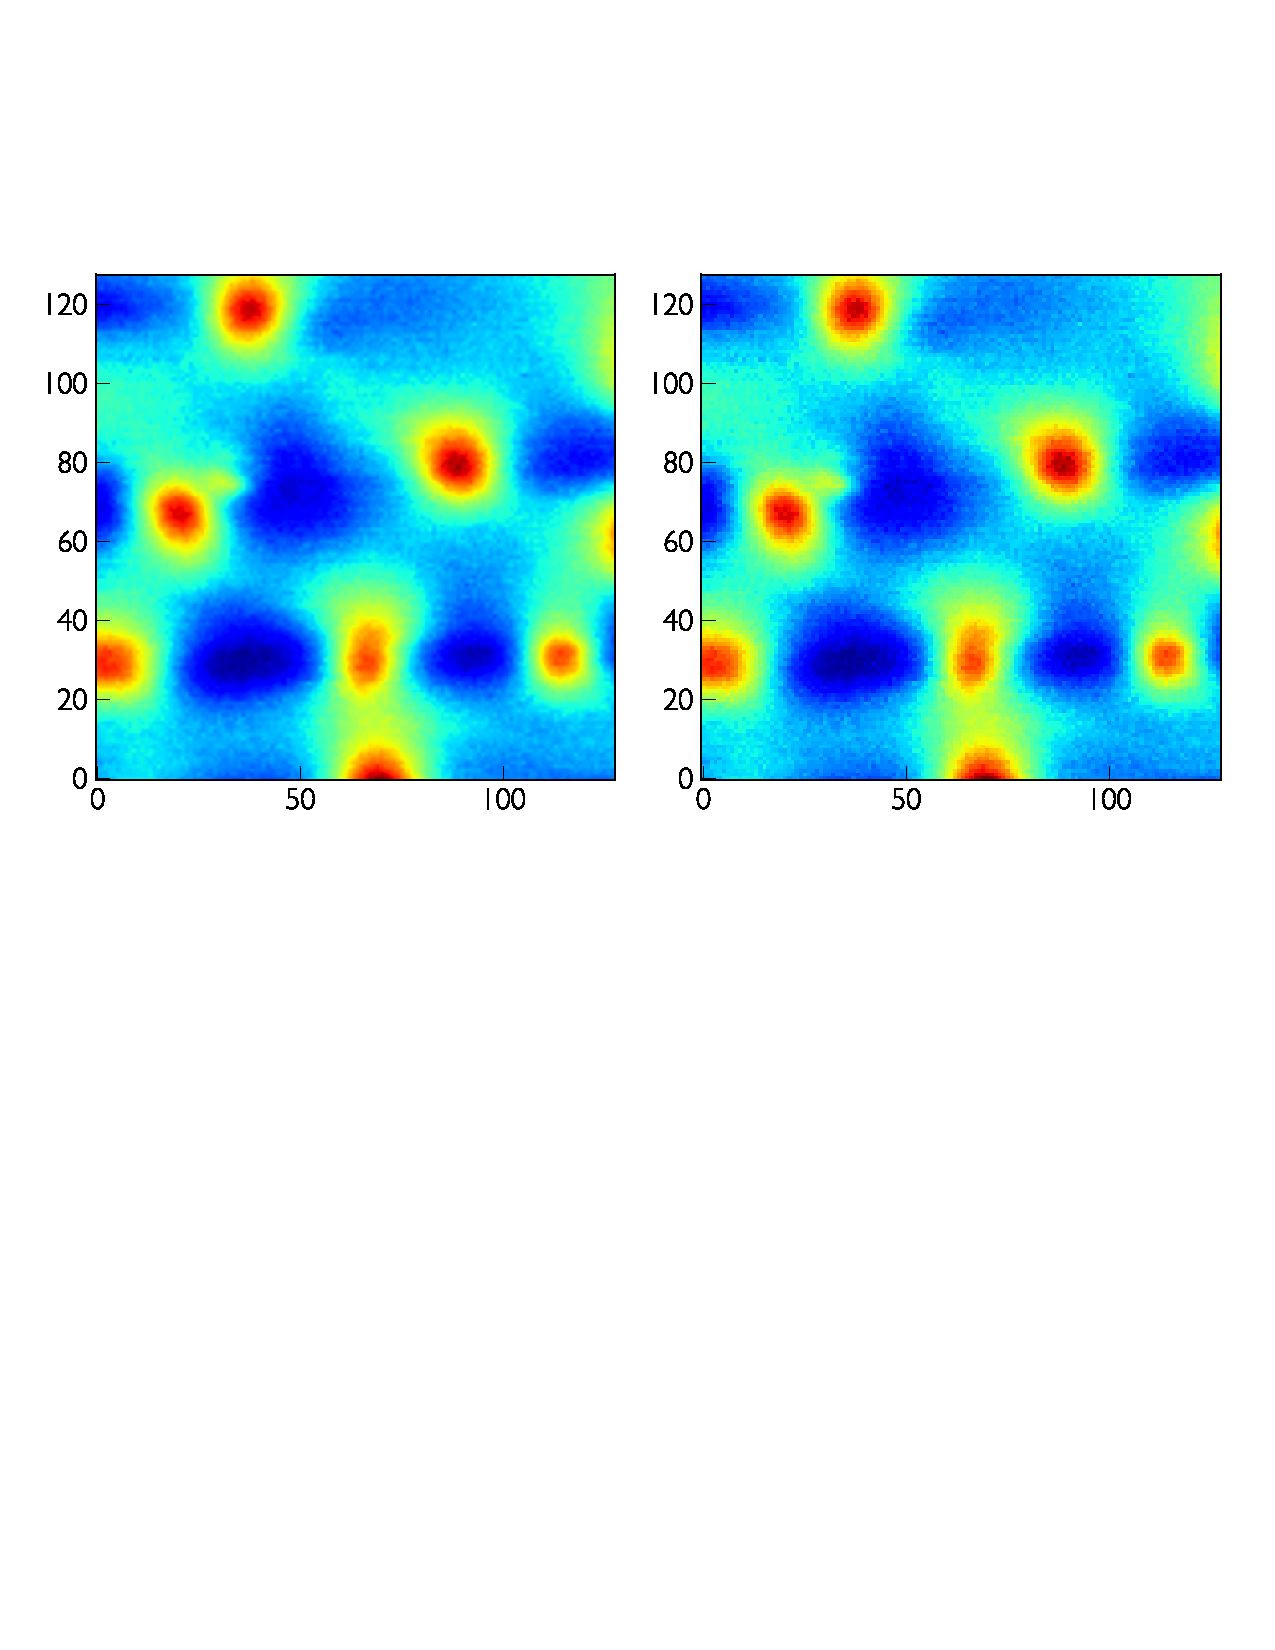
\includegraphics[clip=true,width=\columnwidth]{pixel-compare}
    \caption{Comparison between blurry pixels (dishonest interpolation occurs when the image is processed in Microsoft Powerpoint) vs.\ clean pixels (honest representation is preserved when the image is processed in Python and Adobe Illustrator). MFM images of vortices in NdFeAsO$_{1-x}$F$_x$ \cite{ZhangPRB2015}.}
     \label{fig:pixels}
\end{figure}

\ptitle{Figure file size} Note that faithful representation of images in vector format usually also results in a smaller figures size. This can be important, because some journals and preprint servers have strict size limits on components of a submitted manuscript.

\ptitle{Figure font size} All figure fonts should be at least size \minfont\ in the final publication figure \cite{deBivort}. Note also that san-serif fonts are preferred by most journals (e.g. Arial, Helvetica). To achieve the appropriate font size, please start by measuring the desired final figure size (e.g.\ one or two column width) in the desired journal. Then make a box in Adobe Illustrator (or other program) of exactly the final size, and build your figure within it, using no fonts smaller than size \minfont. Although some journals do prefer that you initially submit your figure at full-page size, you can easily scale up your figure for this purpose. But if you start with a page-size figure and arbitrary font sizes, it becomes harder to later scale it down while maintaining adequate font size.

\vspace{2mm}
\noindent \textbf{Figure checklist:}
\begin{itemize}[label=$\Box$]
\item Use consistent font, at least size \minfont.
\item Label all axes, with units.
\item Each plot should have a legend that describes {\em all} symbols and lines.
\item Each image (or set of same-scale images) should have an accurate length scalebar, with numerical label. (Note that some journals discourage or ``forbid'' superimposing the numerical length on the image. But our goal is clarity: we want the reader to understand the image at a glance, without digging through a lengthy caption to find the necessary number. Journals will generally accept this argument for keeping the number on the image.)
\item Each image (or set of same-palette images) should have a colorbar. The colorbar should be labeled with numerical values and units if possible.
%\item If possible, choose colors that will print well in grayscale. But this is no longer a high priority, since most people read online, or have access to color printers.
\item If using a waterfall plot to display a set of spectra: clearly state the offset of the waterfall plot, or use small horizontal lines to denote the true zero reference for each individual spectrum.
\item The caption should describes all figure sub-parts, in order. Each and every mark on the figure should be described; there should be no mysterious unexplained arrows or other features.
\item If any analysis has been performed (i.e.\ if it's not raw data), then all analysis steps should be clearly divulged, usually in the caption (rather than main text).
\item Clearly explain the origin of all error bars, usually in the caption (rather than main text).
\item For STM images: give setup conditions in the caption ($V_\mathrm{sample}=100$ mV; $R_J=1$ G$\Omega$).
\item For STM spectra: give sample bias modulation in the caption ($V_\mathrm{rms}=2$ mV).
\item For all data: clarify temperature and field conditions in the caption.
\item Appropriately cite all copied figures or data, in the caption of the figure.
\item Use {\tt \textbackslash label\{fig:name\}} within the caption, and use {\tt \textbackslash ref\{fig:name\}} in the paper to refer to it.

\end{itemize}

\section{\label{sec:References}References}

\noindent Referencing should be done using BibTeX.
\begin{itemize}[label=$\Box$]

\item Consistently use reference tags that will be easily recognizable and editable from the tex file, e.g. {\tt AuthorJournalYear}. Suppose you will be citing
Huang {\it et al}, Nano.\ Lett.\ 16, 4224 (2016) \cite{HuangNanoLett2016} and
Huang {\it et al}, Phys.\ Rev.\ B 93, 125129 (2016) \cite{HuangPRB2016}.
Instead of {\tt Huang2016a} and {\tt Huang2016b}, use {\tt HuangNanoLett2016} and {\tt HuangPRB2016}. (Note: You can make these bib tags within Mendeley.)

\item Spend 5 minutes to use find-replace with regular expressions to delete the abstracts, keywords, and other useless information from your bib file, to make it easier to read.
\item Alphabetize the bib entries by author last name, so that it will be easy to notice if there are duplicates. (Note: Mendeley can automatically export them in alphabetical order.)
\item The hyperlink should be generated from the doi, so make sure every bib entry has a valid doi. You should delete the URL field (unless you are specifically citing a website), because it may contain a non-general URL such as \url{https://journals-aps-org.ezp-prod1.hul.harvard.edu/prb/abstract/10.1103/PhysRevB.93.125129}.
\item Check the \LaTeX\ formatting of any special characters in the author's names, e.g. {\tt S\textbackslash\textquotesingle\{a\}nchez}
\item Check the \LaTeX\ formatting in the titles. You need to use extra \{\} around any letters that should be capitalized, e.g.\ {\tt title = \{Quantum Anomalous \{H\}all Effect\} }
\item Chemical formulas should also be enclosed in \{\} so element abbreviations will be capitalized, e.g.\ {\tt title = \{Experiments on \{Bi\$\_2\$Se\$\_3\$\}\}}. Don't use excessively complicated formatting for chemicals. Just put the subscripts in \$\$.
\item Use {\tt longbibliography} in the documentclass at the top of the tex file, so that the title of each paper appears in the references.
\item For most citations, you can just use {\tt \textbackslash cite\{AuthorJournalYear\}}, e.g.\ Jeehoon used conducting force microscopy to measure a metal-insulator transition \cite{KimAPL2010}. But if you're using a superscript citation style, and the citation comes directly after a number or chemical formula, use {\tt Ref.\textbackslash\ \textbackslash onlinecite\{AuthorJournalYear\}} instead to avoid confusion, e.g.\ Jessie measured the pinning force on vortices in NdFeAsO$_{1-x}$F$_x$ (Ref.\ \onlinecite{ZhangPRB2015}).
\item In the compiled PDF, check all the references carefully to make sure they have correctly formatted authors, titles, and hyperlinks.
\end{itemize}

\section{\label{sec:Integrity}Professional Integrity Checklist}

\begin{itemize}[label=$\Box$]
\item Authorship -- are all major contributors and collaborators included? See the American Physical Society guidelines for authorship \cite{APSauthor}.

\item Plagiarism -- have you been careful to distinguish between your own work and ideas, as opposed to those of others?

\item Citations -- have you properly cited prior work, and references that you used?

\item Data Integrity -- have you clearly described the data analysis methods, and justified any data points that were excluded?

\item Image Processing -- have you clearly described any processing that was applied to images?

\item Acknowledgments -- have you given appropriate credit and thanks to collaborators and other individuals or organizations who deserve recognition?

\item Clarity of collaborative structure -- if this is a joint effort, have you identified people who you worked with on this project? Acknowledgments should clearly state who did which parts of the experiment \& analysis, and who wrote the paper.

\item Conflicts of Interest -- do you have any conflicts of interest where you or someone close to you stands to gain, financially or otherwise, from this work?
\end{itemize}

\section{\label{sec:Conclusion}Final Checklist}

\begin{itemize}[label=$\Box$]
\item Think critically about all of your own claims {\em and} about all of the claims made by your coauthors. If you do not understand something that your coauthor has written in the draft, push back until you do understand, then suggest an alternative phrasing to clarify the manuscript or figure.
\end{itemize}

\begin{acknowledgments}
We acknowledge advice from Jessie Zhang and Harry Pirie to produce Fig.\ \ref{fig:pixels}. We also acknowledge a generation of students who have made all of the errors that led to these checklists.
\end{acknowledgments}

\appendix

\section{\label{app:Mendeley}Mendeley}

Mendeley provides a convenient (although not 100\% bug-free) database structure for storing, sorting, and annotating the papers you read. Mendeley also provides an export function to automatically create your bib file. Here are some tips to use Mendeley most effectively.
\begin{enumerate}
\item Download Mendeley: \url{http://www.mendeley.com/}\\ Launch it on your desktop.
\item Set Mendeley options: Make sure your Mendeley database is set correctly to include the DOI (digital object identifier) field. Go to Tools $\rightarrow$ Options $\rightarrow$ Document Details. Scroll down and make sure the DOI box is checked.
\item Import paper: In the upper left corner of Mendeley Desktop, click the drop-down menu for ``Add'' and select the bottom option ``Add Entry Manually''. In the dialog box that pops up, scroll down until you find the DOI field. Paste the DOI into the field, and click the little magnifying glass icon to the right of the field. This will auto-populate all of the relevant paper information such as author names, title, etc., without risk of typos due to manual copying.\\
    \textit{Note 1:} Mendeley also allows you to import directly from a PDF file, and it tries to pull all of the meta-data from the PDF, but the process is imperfect. So it's safest to use the DOI for an error-free import.\\
    \textit{Note 2:} Even if you use the DOI, some journal titles will not import correctly with special characters, so you may need to manually correct.
\item Add tags: It's useful to add tags to help sort your imported papers. For example, if you are going to be writing a manuscript in 2019 on superconductivity, you might add the tag ``sc19'' to all the relevant papers that you will be citing in your manuscript.
\item Export bib file: Select all of the references that you want to include, and go to File $\rightarrow$ Export.  Name your file, and it will add a citation key to each paper (e.g.\ Whitesides2004) and automatically export to a bib file.
\item Resolve redundant citation keys: At this point, you may have several references with the same citation key, e.g.\ Huang2016a and Huang2016b \cite{HuangNanoLett2016, HuangPRB2016}. For your future convenience, you should manually change the redundant citation keys to be more informative, e.g.\ HuangNanoLett2016 and HuangPRB2016. Now re-export the bib file.
\item Open the bib file in your tex file editor. By default, Mendeley exports all fields, including long ones like the abstract. To reduce clutter in your bib file, and make it easier to debug any errors, it's a good idea to remove the abstracts and other unnecessary fields. For example, in WinEdt go to Search $\rightarrow$ Replace, check the regular expressions box, search for ``{\tt <abstract**\textbackslash\},>},'' and replace it with nothing.
\end{enumerate}

\section{\label{app:REVTeX}REVTeX}

\noindent How to install REVTeX 4-2 on Windows for MikTex:
\begin{enumerate}
\item Download REVTeX 4-2:\\ \url{http://authors.aps.org/revtex4/}
\item Unzip the downloaded folder revtex4-2-tds
\item If you don't already have one, create a folder C:\textbackslash TeX-local
\item Copy the four subfolders (bibtex, doc, source, tex) into C:\textbackslash TeX-local
\item From the start menu, open MikTex 2.9 $\rightarrow$ Maintenance (Admin) $\rightarrow$ Settings
\item On the root tab, add the path C:\textbackslash TeX-local
\item On the general tab, click ``Refresh FNDB''
(You may need to close WinEdt, or whatever is using your MikTex installation, in order to properly ``Refresh FNDB''.)
\item Download natbib:\\
\url{http://www.ctan.org/tex-archive/macros/latex/contrib/natbib/}
\item Unzip natbib.
\item Open natbib.ins, and run TeX on it (Shift+Ctrl+T in WinEdt)
\item Open bibentry.ins, and run TeX on it (Shift+Ctrl+T in WinEdt)
%\item You may also need to get two more packages, i.e.\ download from ctan and run TeX on url.ins and textcase.ins
\end{enumerate}

%\newpage % acts like \columbreak for a 2-column doc
\section{\label{app:vectorfig}Vector Graphics}

To create vectorized graphics from python, include {\tt rasterized=True} inside the {\tt imshow} command. Unfortunately, this preference doesn't seem to be allowable as a default in any style sheet, so you need to remember to include it it every time. Then save the python figure as a PDF, which ensures that annotations (like scale bars, axis labels, and lines) remain as vector format, but images retain their proper pixelation. For example:

\begin{minted}[mathescape, linenos]{python}
fig, ax = subplots(1, 1, figsize=[1.8,1.6])
ax.imshow(a.Z, cmap=stmpy.cm.blue2, aspect=1,
  clim=(0,1.4), rasterized=True)
... 
tight_layout(pad=0)
savefig("topo.pdf")
\end{minted}

\noindent Note that some PDF viewers apply their own smoothing to images. For example, MacOS Preview may blur images that look fine in Adobe Illustrator.

\bibliography{Hoffman-example-paper}

\end{document}
